\section{Mathematical Perspective: Support Functions and Imaginative Polytopes}\label{app:imaginative_polytopes}

\subsection{Preliminaries}\label{subsec:support_app}
A \emph{polytope} $P\subseteq\RR^d$ is the convex hull of finitely many vertices in $\RR^d$, or by the Minkowski–Weyl Theorem any finite intersection of finitely many closed halfspaces \citeapp{AppZiegler1995}.
For a polytope $P\subseteq\RR^d$, the \emph{support function} $f_P:\RR^d\to\RR$ is
\begin{align}
    f_P(x) \coloneqq \max_{p\in P} \langle p, x \rangle_{L^2}.
\end{align}
We call the set of points in $P$ that cannot be represented as a nontrivial convex combination of two distinct points in $P$ the vertices of $P$ and denote them by $\text{vert}(P)$.
It is easy to see that
\begin{align}
    f_P(x) \coloneqq \max_{p\in \text{vert}(P)} \langle p, x \rangle_{L^2}. \label{eq:support_function}
\end{align}

A function $f:\mathbb{R}^n \to \mathbb{R}$ is \emph{piecewise linear} (PWL) if there exists a finite polyhedral partition of $\mathbb{R}^n$ such that $f$ is affine on each piece.
It is \emph{continuous piecewise linear} (CPWL) if it is also continuous. 
Note that a function is CPWL exactly if it can be represented by a ReLU network \citeapp{AppArora2018}.

Given the representation \cref{eq:support_function} it is easy to see that the vertices of $P$ correspond one by one to all attainable gradients of $f_P$.
Further, we observe from \cref{eq:support_function} that support functions are convex, continuous, positively homogeneous ($f_P(\lambda c)=\lambda f_P(c)$ for $\lambda\ge 0$), and CPWL. Indeed, the mapping
\begin{align}
    \Phi:\ \mathsf{Polytopes}_d &\longrightarrow \mathsf{CPWL}^+_d, \notag \\
    P &\longmapsto f_P, \label{eq:bijection_cpwl}
\end{align}
is a bijection between $d$-dimensional polytopes and convex, positively homogeneous CPWL functions.

Tropical geometry refers to $P$ as the \emph{Newton polytope} of $f_P$; the correspondence and its learning-theoretic consequences have been exploited in analyses of neural networks and their expressivity \citepapp{AppZhang2018}, \citepapp{AppHaase2023}, \citepapp{AppBrandenburg2024b}.

We call a function $f:\mathbb{R}^n \to \mathbb{R}$ \emph{monotone} in case for any $x_1, x_2 \in \mathbb{R}^d$ with $x_1 \leq x_2$ (understood elementwise) one has $f(x_1) \leq f(x_2)$.

As shown in \cref{app:fundamental}, the split-streams $g$ and $h$ defined in \cref{sec:method} are positively homogeneous monotone convex CPWL functions and therefore possess corresponding Newton polytopes $P_g$ and $P_h$ by the bijection in \cref{eq:bijection_cpwl}.
It is easy to see that by the monotonicity of $g$ and $h$ all points in $P_g$ and $P_h$ have non-negative coordinates as the gradients of $g$ and $h$ are non-negative.
\TODO{GL: Ist die folgende Aussage nicht auch schon im Abschnitt A.1 implizit?}
\TODO{JZ: Ich glaube, ich habe den remark zu positiven vertices wieder gelöscht gehabt. Ich habe das Theorem hinzugefügt um klarzumachen, dass unsere Intuition zu positiven Gradienten nicht nur NNs mit positiven Gewichten betrifft. Das Argument ist natürlich sehr einfach und ich finde es auch implizit in der maximum formulierung der support funktion.}
\begin{theorem} \label{thm:monotonicity_positive_gradients}
    Let $g: \ \mathbb{R}^{d} \longrightarrow \mathbb{R}$ be a monotone and CPWL function. Then $\nabla g \geq 0$, \ie all its attainable gradients are non-negative.
\end{theorem}

\begin{proofref}{Theorem}{thm:monotonicity_positive_gradients}
    Assume for a contradiction that there is $x \in \mathbb{R}^d$ and $j \in [d]$ such that the $j$th component of the gradient at $x$ is negative, \ie $\left( \frac{\partial g}{\partial x} \right)_j < 0$.
    As $g$ is piecewise linear, there is $\epsilon > 0$ such that $g$ is linear in the $\epsilon$-ball around $x$. However for $\tilde{x} \coloneqq x - \frac{\epsilon}{2} e_j$ one finds $\tilde{x} \leq x$ but $f\left( \tilde{x} \right) > f(x)$. This contradiction concludes the proof of \cref{thm:monotonicity_positive_gradients}.
\end{proofref}

\subsection{Imaginative Polytopes}\label{subsec:imaginative_polytopes}
In the ablation study \cref{app:ablation} we observe that the gradients of the split-pair show greater robustness than the gradients of the original model, \ie small input perturbation results in less perturbed gradients.
We want to argue that indeed the non-negativity of the split-stream gradient could be one important reason for this behavior.
Indeed, as the split-stream outputs are just the maximum scalar products of the input with all attainable gradients respectively, see \cref{eq:support_function}, the non-negativity of the gradients results in more stable gradients due to no cancellation in the scalar product. 
Further, any jump of the gradients in the original network does not force both gradients of $g$ and $h$ to jump, but only one of them.

Secondly, we observe dramatically better localization properties of the split-pair gradients compared to the original gradients. Again, we find it intuitive that positive gradients show better focus on salient image regions as no cancellation can happen.

Because the vertices of $P_g$ and $P_h$ empirically align closely with salient image structures we term them \emph{Imaginative Polytopes}: intrinsic geometric objects induced by ReLU networks that summarize the model's learned visual features and thereby help to explain how common vision models envision and ``imagine'' the world. Their vertices correspond to distinct activation patterns and represent the fundamental ``prototypes'' that the network has learned to distinguish different input features.
We visualize the $g$-stream gradient of VGG16 with respect to the ``dragonfly'' class output logit for four ImageNet test images in \cref{fig:imaginative_polytope}, where we applied backward pass shifting with $\alpha=0.25$. We remark that the $h$-stream gradient looks very similar, as it only differs to the $g$-stream gradient in the gradient of the original VGG model -- for this reason we linked the $g$-stream gradient visualizations also with corresponding $h$-stream gradients.

\begin{figure}[htbp]
    \centering
    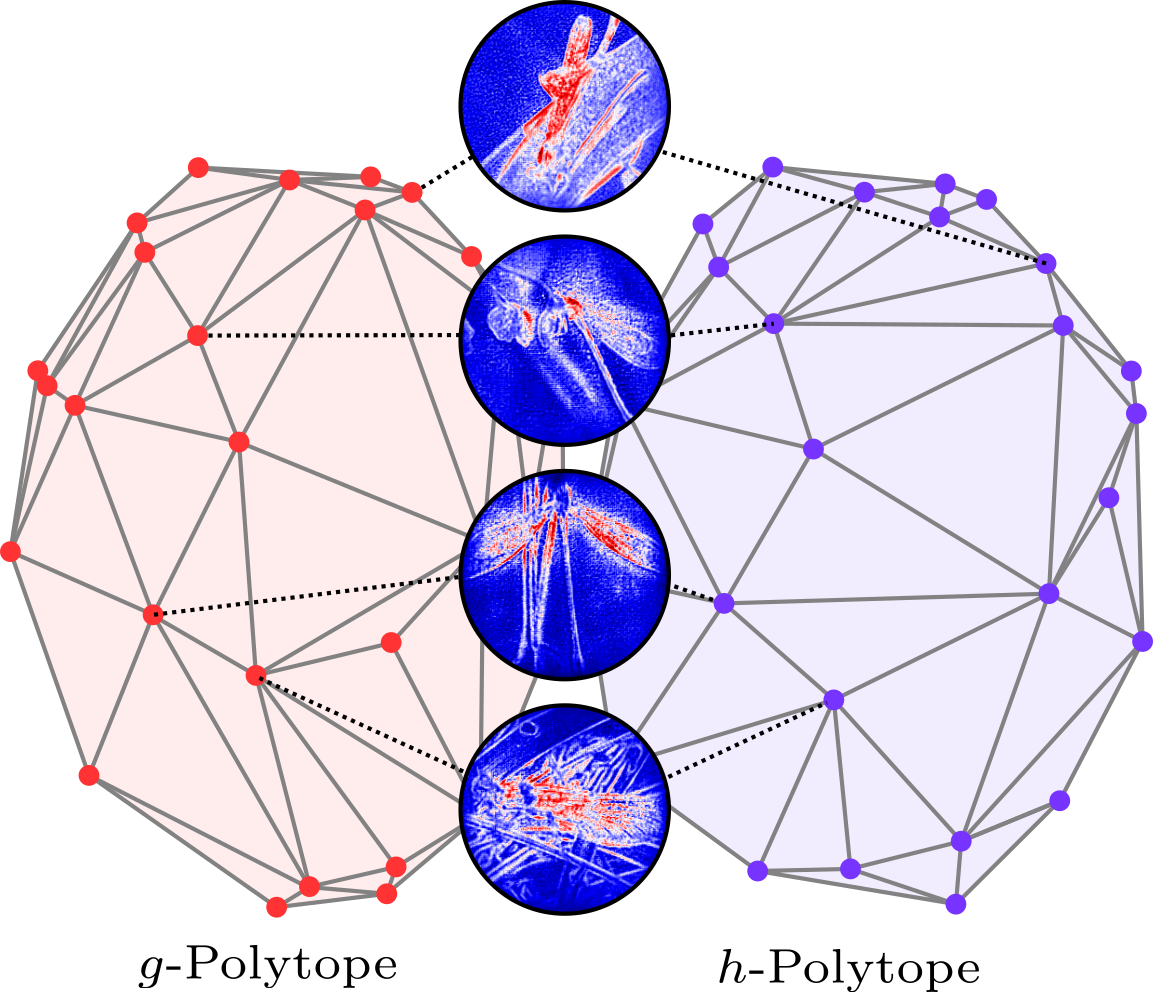
\includegraphics[width=0.6\textwidth]{figures/imaginative_polytope.png}
    \caption{Concept visualization of the imaginative polytopes corresponding to VGG's dragonfly class output neuron. The polytope's vertices represent the $g$-stream and $h$-stream gradients respectively, revealing learned visual prototypes.}
    \label{fig:imaginative_polytope}
\end{figure}